\documentclass[times, twoside]{PosWhiPap}
\usepackage{blindtext}



% Please give the surname of the lead author for the running footer
\leadauthor{S.~Fucini {\it et al.}}  

\begin{document}

\title{Deeply virtual Compton scattering off Helium nuclei with positron beams}
\shorttitle{Positrons on He targets}

% Use letters for affiliations, numbers to show equal authorship (if applicable) and to indicate the corresponding author
%\author[1,\Letter]{Ricardo Henriques}
\author[1]{S.~Fucini}
\author[2]{M.~Hattawy}
\author[1]{M.~Rinaldi}
\author[1]{S.~Scopetta}


\affil[1]{Dipartimento di Fisica e Geologia, Università degli studi di Perugia, 
and INFN, sezione di Perugia, via A. Pascoli snc, 06123, Perugia, Italy}

\affil[2]{Old Dominion University, Norfolk, Virginia 23529, USA.}


\maketitle

%TC:break Abstract
%the command above serves to have a word count for the abstract
\begin{abstract}
%\blindtext
The relevance of using positron beams in deeply virtual Compton scattering (DVCS) off $^4$He and $^3$He 
   is addressed. The way the so-called $d-$term could be extracted from the 
   real part of the relevant Compton form factor, using as an example coherent 
   DVCS on $^4$He, is summarized, and the importance and novelty of this measurement is described. Analogous measurements are addressed for $^3$He tagets,
   which could be very useful even in a standard unpolarized setup, measuring beam spin asymmetries and charge beam asymmetries only.
   The role of incoherent  
   DVCS processes, in particular tagging the internal target by measuring slow recoiling nuclei,  and the unique possibility offered by positron beams for the 
   investigation of Compton form factors of higher twist, are also  briefly 
   addressed.
\end {abstract}
%TC:break main
%the command above serves to have a word count for the abstract

%\begin{keywords}
%bla | bla | bla | bla
%\end{keywords}

%\begin{corrauthor}
%\texttt{r.henriques{@}ucl.ac.uk}
%r.henriques\at ucl.ac.uk
%\end{corrauthor}


\section*{Introduction}
{
The possibility to shed 
   light on the EMC effect, i.e., the nuclear modifications of the nucleon 
   parton structure \cite{Dupre:2015jha, Cloet:2019mql}, as well as
   the possibility to distinguish coherent and incoherent 
   channels, experimentally recently demonstrated by 
   the CLAS collaboration at JLab using a $^4$He gaseous target
     \cite{Hattawy:2017woc, Hattawy:2018liu},
   have produced, in recent years, a growing interest on nuclear deeply virtual Compton scattering (DVCS). Let us analyze
   the imact that measurements of positron initiated DVCS on $^4$He and $^3$He may have, separately for the coherent an incoherent channels}.

\section*{Coherent DVCS}
To fix the ideas on how positron beams could help in this field, 
let us think first to coherent DVCS off $^4$He.
%As observed for the nucleon target before in this White Paper,
%positrons allow a precise extraction of the Re CFF.
We recall that $^4$He has only one chiral even Compton Form Factor (CFF), corresponding
to one generalized parton distribution (GPD) at 
   leading twist. In the EG6 experiment of the CLAS collaboration
   \cite{Hattawy:2017woc}
   the crucial measured
observable was the single-spin asymmetry
$A_{LU}$, which can be extracted from the reaction yields with the two electron
helicities ($N^{\pm}$):
\begin{equation}
A_{LU} = \frac{1}{P_{B}} \frac{N^{+} - N^{-}}{N^{+} + N^{-} },
\end{equation}
where $P_{B}$ is the degree of longitudinal polarization of the incident 
electron beam.
 In EG6 kinematics, the cross section of real photon electroproduction is 
   dominated by the BH contribution, while the DVCS contribution is very small.  
   However, the DVCS contribution is enhanced in the observables sensitive to 
   the interference term, {\it e.g.} $A_{LU}$, which depends on the
azimuthal angle $\phi$ between the $(e,e^\prime)$ and 
   $(\gamma^*,^4$He$^\prime)$ planes. The asymmetry $A_{LU}$ for a spin-zero 
   target can be approximated at leading-twist as
\begin{equation}
A_{LU}(\phi) = 
\frac{\alpha_{0}(\phi) \, \Im m(\mathcal{H}_{A})} 
{den(\phi)} \, ,
\end{equation}
\begin{eqnarray}
den(\phi) & = & 
\alpha_{1}(\phi) + \alpha_{2}(\phi) \, \Re e(\mathcal{H}_{A}) 
\nonumber
\\
& + & \alpha_{3}(\phi) \, 
\big( \Re e(\mathcal{H}_{A})^{2} + \Im m(\mathcal{H}_{A})^{2} \big)\, .
\label{boh}
\end{eqnarray}
The kinematic factors $\alpha_i$ are known (see, e.g., Ref.  
\cite{Belitsky:2001ns,Belitsky:2008bz}). 
In the experimental analysis,
using the different contributions proportional to
$\sin(\phi)$ and 
$\cos(\phi)$ in \eqref{boh},  both the real and 
imaginary parts of the so-called Compton Form Factor $\mathcal{H}_{A}$,
$\Re e(\mathcal{H}_{A})$ and $\Im m(\mathcal{H}_{A})$, respectively,
have been extracted by fitting the $A_{LU}(\phi)$ distribution. 
Results of the impulse approximation calculation  
of Ref. \cite{Fucini:2018gso} are shown together with the data 
of Ref. \cite{Hattawy:2017woc} in Figs. \ref{uno} and \ref{due}.
Big statistical errors are seen everywhere in the data but the extracted $\Re 
e(\mathcal{H}_{A})$ is less precise than $\Im m(\mathcal{H}_{A})$, due to the small 
coefficient $\alpha_2$ in \eqref{boh}.

\begin{figure}[tbhp]
\centering
\includegraphics[width=.7\linewidth, angle=270]{Figures/imxb.eps}
\caption{The imaginary part of the CFF measured in coherent DVCS off $^4$He.
Data from Ref. \cite{Hattawy:2017woc}; calculations (red crosses) from
Ref. \cite{Fucini:2018gso}}.
\label{uno}
%\end{figure}
%\begin{figure}%[tbhp]
%\centering
\includegraphics[width=.7\linewidth, angle=270]{Figures/rexb.eps}
\caption{
The real part of the CFF measured in coherent DVCS off $^4$He.
Data from Ref. \cite{Hattawy:2017woc}; calculations (red crosses) from
Ref. \cite{Fucini:2018gso}.
}
\label{due}
\end{figure}

Forth-coming data form JLab 12 with electron beams, using also the detector system
developed by the ALERT run-group \cite{Armstrong:2017wfw}, will obtain smaller 
errors. Realistic theoretical calculations are possible for light nuclei and could help 
to unveil an exotic behavior of the real and imaginary part of $\mathcal{H}_{A}$.
Nonetheless, the extracted $\Re e(\mathcal{H}_{A})$ will be always less precise than
$\Im m(\mathcal{H}_{A})$, intrinsically, due to the small coefficient $\alpha_2$
in \eqref{boh}.
A precise knowledge of $\Re e(\mathcal{H}_{A})$ for light nuclei would be instead crucial.
Positrons beams would guarantee this achievement: as a matter of fact, combining data for asymmetries measured 
using electrons and positrons the role of $\Re e \mathcal{H}_{A}$ would be 
directly accessed. Let us recall how it is possible.

One should notice that, between the quantities appearing in the above
equations and the cross sections defining the generic photo-$e^\pm$production 
cross section in the following schematic general expression, previously given 
in this White Paper,
\begin{eqnarray}
\sigma^e_{\lambda 0}  & = & \sigma_{BH} + \sigma_{DVCS} + \lambda \tilde \sigma_{DVCS} 
\nonumber
\\
& + & e\sigma_{INT} + e \lambda \tilde \sigma_{INT} \, ,
\label{gen}
\end{eqnarray}
the following relations hold:
\begin{eqnarray}
\sigma_{BH} & \propto & \alpha_1(\phi)\, ,
\nonumber \\
\sigma_{DVCS} & \propto &   \alpha_{3}(\phi) 
\big( \Re e(\mathcal{H}_{A})^{2} + \Im m(\mathcal{H}_{A})^{2} \big) \, ,
\nonumber \\
\sigma_{INT} & \propto & \alpha_{2}(\phi) \, \Re e(\mathcal{H}_{A}) \, ,
\nonumber \\
\tilde \sigma_{INT} & \propto & \alpha_{0}(\phi) \, \Im m(\mathcal{H}_{A}) \, ,
\end{eqnarray}

while $\tilde \sigma_{DVCS} $ is proportional to a term kinematically suppressed
at JLab kinematics, dependent on higher twist CFFs. 

From a combined analysis of data taken with polarized electrons and/or 
positrons, one could access all the five cross sections in \eqref{gen}.
{\bf We stress in particular that, using just unpolarized electrons and positrons, $\Re 
e(\mathcal{H}_{A})$ would be directly accessed, building charge beam asymmetries}. Let us briefly 
analyze why the knowledge of $\Re e\mathcal{H}_{A}$ would be very
important for nuclei. Formally one can write,
for the quantities $\Re e(\mathcal{H}_{A})$ and $\Im m \mathcal{H}_{A}$
shown in Figs.~\ref{due} and \ref{uno} respectively \cite{Guidal:2013rya}:
\begin{equation}
\Re e \mathcal{H}_{A} (\xi,t) \equiv 
{\cal P} \int_0^1 dx H_+(x,\xi,t) C_+(x,\xi) \, ,
\label{ReC}
\end{equation}
and
\begin{equation}
  \Im m \mathcal{H}_{A} = -\pi H_+(\xi,\xi,t)  \, ,
\end{equation}
with:
\begin{equation}
    H_+ = H(x,\xi,t)-H(-x,\xi,t) \, ,
\end{equation}
amd
\begin{equation}
    C_+(x,\xi) = \frac{1}{x+\xi}+\frac{1}{x-\xi} \, ,
\end{equation}

with $H(x,\xi,t)$ the chiral even, leading twist generalized parton distribution
(GPD).


Besides, it is also known that $\Re e(\mathcal{H}_{A})$ satisfies a once 
subtracted dispersion relation at fixed $t$ and can be therefore related
to $\Im m \mathcal{H}_{A}$, leading to 
\cite{Anikin:2007yh,Diehl:2007jb,Radyushkin:2011dh,Pasquini:2014vua}
\begin{equation}
\Re e \mathcal{H}_{A} (\xi,t) \equiv
{\cal P} \int_0^1 dx H_+(x,x,t) C_+(x,\xi)
- \Delta(t) \, .
\label{disp}
\end{equation}

One notices that, in contrast to the convolution integral defining the real 
part of the CFF in \eqref{ReC}, where the GPD enters for unequal values of its 
first and second argument, the integrand in the dispersion relation
corresponds to the GPD where its first and second arguments are equal.
The subtraction term $\Delta(t)$ can be related to the so-called $d-$term and
accurate measurements, supplemented by precise calculations, would allow therefore to study
this quantity in nuclei, for the first time.
This $d-$term, introduced initially to recover 
polinomiality in DDs approaches to GPDs modelling \cite{Polyakov:1999gs},
has been related to the form factor of the QCD energy momentum tensor (see e.g. Ref.  
\cite{Polyakov:2018zvc}). It encodes information on the distribution of forces 
and pressure between elementary QCD degrees of freedom in the target. For
nuclei, it has been predicted to behave as $A^{7/3}$ in a mean field scheme, 
either in the liquid drop model of nuclear structure \cite{Polyakov:2002yz}
or in the Walecka model \cite{Jung:2014jja}. None of these approaches makes 
much sense for light nuclei, for which accurate realistic calculations are possible. 
Using light nuclei one would therefore explore, at the parton 
level, the onset and evolution of the mean field behavior across the
periodic 
table, from deuteron to $^4$He, whose density and binding are not far
from those of finite nuclei.
\vskip 0.2cm
In this sense, coherent DVCS off $^3$He targets acquire an important role: an intermediate 
behavior is expected between that of the almost unbound deuteron system and 
that of the deeply bound alpha particle. The formal description of coherent DVCS
off $^3$He follows that already presented for the proton, a spin one-half target, in terms of CFFs
and related GPDs. Properly
defining spin dependent asymmetries. Realistic theoretical calculations
are available for GPDs 
\cite{Scopetta:2004kj,Scopetta:2009sn,Rinaldi:2012ft,Rinaldi:2012pj} and are in 
progress for the relevanto CFFs, cross sections and asymmetries, representing
an importanmt support to the planning of measurements.
{\bf One should notice that, while the use of $^3$He, either longitudinally or transversely polarized,
would represent at the moment a challenge, either with electron or positron beams, 
beam charge asymmetries, built using
electron and positron data, would represent, even with unpolarized $^3$He targets and unpolarized beams, a possible access to
$\Re e \mathcal{H}_{A} (\xi,t)$,
as previously described for $^4$He, with the same potential to explore the "d-"term.}

\section*{Incoherent DVCS}
{\bf
A subject aside is represented by incoherent DVCS off He nuclei, i.e.,
the process where, in the final state, the stuck proton is detected, its CFFs accessed, its GPDs, in principle, extracted and, ultimately, its tomography obtained.
This would provide a pictorial representation of the realization of the EMC effect and a great progress towards the understanding of its dynamical origin.
As already stressed, this channel has been successfully isolated by the EG6 experiment of the CLAS collaboration at JLab \cite{Hattawy:2018liu} and a first glimpse at the parton structure of the bound proton in the transverse coordinate space is therefore at hand (see the recent impulse approximation calculation in Ref. \cite{Fucini:2019xlc} for a theoretical description
of the recent data with conventional realistic ingredients).
The program at JLab 12 includes an improvement of the accuracy of these measurements, in particular, for the first time in DVCS, tagging the struck nucleon using the detector
developed by the ALERT run group \cite{Armstrong:2017zcm}.
This would allow to keep possible final state interactions, relevant in principle in this channel, under control.
Measurements performed with 
electron and positron beams  would allow for example the measurement of the $d-$term for the bound nucleon, either proton in $^3$He (tagging 2H from DVCS on $^3$He)  or in $^4$He (tagging $^3$H from 
DVCS on $^4$He) or neutron in $^4$He (tagging $^3$He from DVCS on $^4$He). Modifications 
of the $d-$term of the nucleon in the nuclear medium, studied e.g. in
Ref.
\cite{Jung:2014jja}, would be at hand, as well as a glimpse at the structure of the neutron
in the transverse plane, complementary to that obtained with deuteron targets.}

\section*{Beyond a chiral even GPDs description of DVCS on $^4$He}

{\bf As a last argument,
we note that, from the measurement of 
beam spin asymmetries built using 
cross sections measured with polarized electrons and positrons
in coherent DVCS off $^4$He, the 
cross sections $\tilde 
\sigma_{DVCS}$
and $\tilde 
\sigma_{INT}$
appearing in \eqref{gen},
could be independently accessed.
This would allow,
for the first time, 
to study the other leading twist CFF of a spinless target,
the so called  gluon transversity GPD $H_T$, giving a corresponding
name to the CFF ${\cal{H}}_T$, appearing in
$\tilde  \sigma_{DVCS}$. In Ref. 
\cite{Belitsky:2008bz}, it is shown how
the contribution of ${\cal{H}}_T$ to the cross section
occurs through an interference between twist-two
and effective twist-three CFFs. A first glimpse at this complicated interrelation
would be obtained for a spin-less target, in particular for a nuclear target,
for the first time.
As for any other gluon-sensitive observable, data for the cross section
$\tilde  \sigma_{DVCS}$ would be a perfect tool to study gluon dynamics in nuclei. For example, a comparison with calculations performed in an Impulse Approximation scheme, where the relevant nuclear degrees of freedom
are colorless nucleons and mesons, with gluons confined within them, would
have the potential to expose possible exotic gluon dynamics in nuclei.
This would be a pretty new possibility, complementary to that planned at JLab
with 12 GeV, using exclusive vector meson electroproduction off
$^4$He \cite{Armstrong:2017zcm}.
Such an interersting behavior would be very hardly seen using electrons only,
due to the strong kinematical suppression of $\tilde  \sigma_{DVCS}$ with respect to
the other contributions in \eqref{gen}.
}

\section*{Conclusions}
{\bf
The unique possibilities offered by the use of positron beams in DVCS off three- and four-body nuclear systems have been reviewed. Summarizing, we can conclude that the main advantages will be:
\begin{itemize}
    \item in coherent DVCS off $^3$he and $^4$He, using polarized electrons and unpolarized positrons,
    the real part of the chiral even unpolarized CFF would be measured with a precision comparable to that of the imaginary part, providing a tool for the study of the so called $d$ term and to the distribution of pressure and forces between the partons in nuclei, a new way to look at the nuclear medium modifications of nucleon structure; 
    \item in incoherent DVCS off $^3$He and $^4$He, possibly tagging slow recoiling nuclear systems, the same programme could be run for the bound proton and neutron;
    \item using polarized $^3$He targets, a more complicated setup for the moment, spin dependent and parton helicity flip CFFs would be accessed for the first time for a nucleus, in both their real and imaginary parts;
    \item coherent DVCS off $^4$He, initiated with polarized positrons, would allow a first analysis of nuclear chiral odd CFFs and GPDs, with higher twist contaminations suitable to temptatively explore gluon dynamics in nuclei.
\end{itemize}
A programme of nuclear measurements with positron beams would represent therefore an exciting complement to the experiments planned with nucleon targets. 
}





%\section*{Results}

%Just for kicks here's a citation \cite{Gustafsson2016}. And a %reference to a supplement \cref{note:Note1}. And %\nameref{note:Note1}.
%\Blindtext





%\Blindtext

%Figure \ref{fig:computerNo} shows an example of how to insert a column-wide figure. To insert a figure wider than one column, please use the \verb|\begin{figure*}...\end{figure*}| environment. Figures wider than one column should be sized to 11.4 cm or 17.8 cm wide. Use \verb|\begin{SCfigure*}...\end{SCfigure*}| for a wide figure with side captions.

%\Blindtext \Blindtext \Blindtext

%\section*{Conclusions}

%$blablaba \ref{fig:computerNo} 
%\blindtext

%\subsection*{Blabla} 
%\blindtext

%\section*{Conclusions}

%blablaba \ref{fig:computerNo}
%\blindtext

%\begin{acknowledgements}
%\blindtext
%\end{acknowledgements}

\newpage

\section*{Bibliography}
\bibliography{MyWPCont}

%% You can use these special %TC: tags to ignore certain parts of the text.
%TC:ignore
%the command above ignores this section for word count
\onecolumn
\newpage

%\section*{Word Counts}
%This section is \textit{not} included in the word count. 
%\subsection*{Notes on Nature Methods Brief Communication}
%\begin{itemize}
%\item Abstract: 3 sentences, 70 words.
%\item Main text: 3 pages, 2 figures, 1000-1500 words, more figures possible if under 3 pages
%\end{itemize}

%\subsection*{Statistics on word count}
%\detailtexcount
%\newpage

 %%%%%%%%%%%%%%%%%%%%%%%%%%%%%
%% Supplementary Information %
%%%%%%%%%%%%%%%%%%%%%%%%%%%%%%
%\captionsetup*{format=largeformat}
%\section{Full list of authors and affiliations} \label{note:Note1} 

%S.~Fucini$^a$, M.~Hattawy$^b$, M.~Rinaldi$^a$, S.~Scopetta$^a$  

%\begin{center}

%{\it
%$^a${Dipartimento di Fisica e Geologia, Università degli studi di Perugia, and 
%   INFN, sezione di Perugia, \\
%   via A. Pascoli snc, 06123, Perugia, Italy}

% $^b${Old Dominion University, Norfolk, Virginia 23529, USA.}
% }
%\end{center}

%%TC:endignore
%%the command above ignores this section for word count


\end{document}
